\subsubsection{Explicación}
Esta es una de las formas más sencillas de abordar el problema del viajante.

Primero escogeremos una ciudad de inicio. Después de ello calculamos las distancias de esa ciudad al resto y escogemos la más cercana.
En el programa usado de ejemplo la clase grafo almacena los puntos (sus coordenadas) y la matriz de adyacencia del grafo, por tanto no 
tendremos que calcular repetidas veces las distancias.

\begin{figure}[htb] 
	\centering
	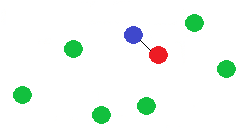
\includegraphics[width=1.75\textwidth]{./Imagenes/vecino1.png}
	\caption{Eligiendo punto de inicio en azul} 
\end{figure}

Estamos utilizando un enfoque greedy, calculando una solución óptima en cada paso local, con la experanza de llegar a una solución que se
acerque al óptimo (o lo sea, en algunos casos). Repetimos el mismo paso con cada punto:

\begin{figure}[htb] 
	\centering
	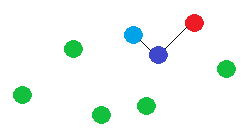
\includegraphics[width=1.75\textwidth]{./Imagenes/vecino2.png}
	\caption{Tercer vértice} 
\end{figure}

\begin{figure}[htb] 
	\centering
	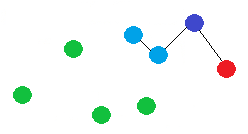
\includegraphics[width=1.75\textwidth]{./Imagenes/vecino3.png}
	\caption{Cuarto vértice} 
\end{figure}

\begin{figure}[htb] 
	\centering
	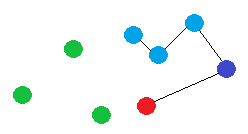
\includegraphics[width=1.75\textwidth]{./Imagenes/vecino4.png}
	\caption{Quinto vértice} 
\end{figure}

\begin{figure}[htb] 
	\centering
	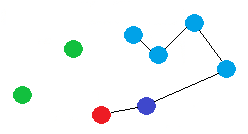
\includegraphics[width=1.75\textwidth]{./Imagenes/vecino5.png}
	\caption{Sexto vértice} 
\end{figure}

\begin{figure}[htb] 
	\centering
	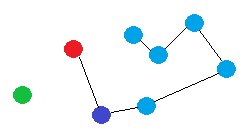
\includegraphics[width=1.75\textwidth]{./Imagenes/vecino6.png}
	\caption{Séptimo vértice} 
\end{figure}

\begin{figure}[htb] 
	\centering
	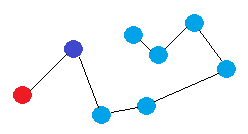
\includegraphics[width=1.75\textwidth]{./Imagenes/vecino7.png}
	\caption{Octavo y último vértice} 
\end{figure}

No debemos olvidar incluir el camino del último vértice al inicial, ya que forma parte del problema y hay que sumar también esa distancia.

\begin{figure}[htb] 
	\centering
	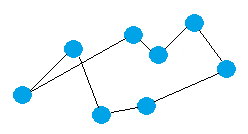
\includegraphics[width=1.75\textwidth]{./Imagenes/vecino8.png}
	\caption{Recorrido vecino más cercano} 
\end{figure}

El número de caminos (aristas) que debe recorrer coincide con el número de ciudades.
Esta solución es muy rápida de implementar y nos da una solución cercana a la óptima, pero no tiene porque ser la óptima.

\subsubsection{Eficiencia}
Siendo $n$ el número de ciudades por las que nuestro viajero debe pasar, denotamos cada una como $x_i=(i_a, i_b)$, $i\in\{0,1,...,n-1\}$
Definimos $\phi (x):\mathbb{N} \rigtharrow \mathbb{N}$ como la función que dado un vértice o ciudad $x_i$ nos devuelve el 
índice de la ciudad más cercana, siendo su eficiencia lineal. Una vez iniciado el algoritmo nos interesará que solamente calcule
el mínimo de las distancias con las ciudades que aún no ha recorrido.
\[\phi(x_i) = \{j \in\{0,1,...,n-1\}-\{i\} : min\{dist(x_i, x_j)\} \}\]
donde 
\[ dist(x_i, x_j) = \sqrt{(i_a-j_a)^2+(i_b-j_b)^2} \]

Tenemos que pasar por las $n$ ciudades, por lo que podríamos pensar que su eficiencia es:
\[O(n) = \sum_{k=0}^{n-1} \phi(x_k)  \]

Sin embargo el algoritmo que buscamos no es tan bueno como el cuadrático, ya que tenemos una restricción. En cada paso el cálculo
del mínimo tiene que comprobar que la nueva ciudad no forme ciclo (pasaríamos dos veces por la misma ciudad).
Por tanto definimos $A$ como el conjunto de los índices de las ciudades que no han sido visitadas aún.
\[\phi '(x_i) = \{j \inA : min\{dist(x_i, x_j)\} \ y \ no \ forme \ ciclos \}\]

Comprobar si una ciudad forma ciclos es lineal, por lo que tenemos que $\phi '(x_i)$ es cuadrático.
La eficiencia del vecino más cercano queda definida como sigue:

\[ \sum_{k=0}^{n-1}\phi ' (x) \implies O(n) = n^3\]

\subsubsection{Gráficas}
